% =================
% Bots
% =================
\subsection{Bot/Shell}
\label{sec:specie-bots}

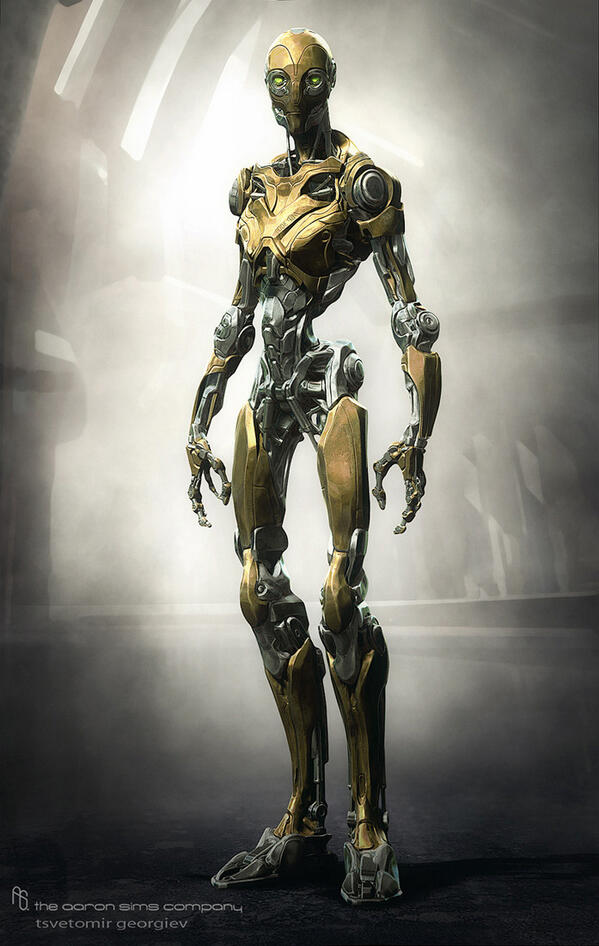
\includegraphics[width=\linewidth]{BEzZuPdCEAAgcr8}

Bots, Ghosts, Shells. These are the names given to the digital constructs that work and live beside organics. Many organics do not trust these artificial "beings" because they fear that the robots will take their jobs (and even murder them).

To create a Bot, Ghost or AGI character, please refer to the \textit{\hyperref[sec:rules-creation]{Character creation section}}\\

\begin{genericsection}{"Weak" AI \& Bots}
Most Bots are limited to a singular purpose by their programming, and are designed to operate in a single chassis optimised for their task. They do have advanced Neural Network pathways, fuzzy systems and deep memory to help them overcome obstacles and solve problems related to their duties. A few advanced models even have a limited sense of self, blurring the lines between normal Bots and an AGI.\\

Robots limited in this way are known as "weak AI".
\end{genericsection}

\begin{genericsection}{AGI, or true AI}
An Artificial General Intelligences (AGI) is loosely defined as a digital entity that has fully developed the ability to understand that other people, creatures and objects in the world may have thoughts, emotions and motives that can affect it's own behavior. It also has full self-awareness, and can at times seem almost indistinguishable from normal organics. Scholars debate whether these digital entities can actually have "feelings" or other properties that are associated with organic beings.
\end{genericsection}

\begin{genericsection}{Ghosts and their Shells}
There are some organic individuals who have made the transition to become fully digital. These individuals, known as Ghosts, have chosen to digitise their conciousness and upload themselves into artificial bodies known as Shells. Many in society believe that these digitised conciousnesses have lost their basic "humanity", and are indistinguishable from an AGI.
\end{genericsection}

\begin{genericsection}{The Cortical Stack}
The Cortical Stack is the most important piece of hardware for any digital entity. The Stack is where their "conciousness" is stored. The entity can usually retain their memories and personality when their Stack is transferred to a new chassis (although "weak" AI cannot operate a chassis significantly different from their own due to their limited programming).

It also should be noted that it is \textbf{highly illegal} to run multiple copies of yourself throughout most civilised planets. This is because generally the digital clones try to "murder" each other so that they can become the official version of the consciousness (among other fears).
\end{genericsection}

\begin{genericsection}{Becoming the System}
A Ghost or AGI can sometimes inhabit other digital systems such as servers and computers. Keep in mind the following:
\end{genericsection}

\begin{itemize}
  \item \textbf{Hardware}: Not all computer systems have the hardware needed to hold and operate a Ghost or AGI. In these cases it is better to hack the system instead\\
  \item \textbf{Limited Sensors}: Most systems do not even bother with audio/visual input, relying on a user to type in commands through a terminal or keyboard\\
  \item \textbf{Illegal}: Unless expressly given permission to do so, and the existing system does not already have an AI.\\
\end{itemize}
